\documentclass[11pt]{scrartcl}

\title{Template}
\author{Silvan Adrian \\ Fabian Binna}
\date{\today{}}

\usepackage[ngerman]{babel}
\usepackage[automark]{scrpage2}
\usepackage[colorlinks = true,
linkcolor = black]{hyperref}
\usepackage{color}
\usepackage[normalem]{ulem}
\usepackage{scrpage2}
\usepackage{graphicx}
\usepackage{tabularx}
\graphicspath{ {../22_Grafiken/01_Logo/}{images/}{../../22_Grafiken/01_Logo/} }
\pagestyle{scrheadings}

\clearscrheadfoot
\ihead{
\includegraphics[scale=0.3]{SDDC}}
\ohead{Projekt: SDDC}
\ifoot{Template}
\cfoot{Version: 1.01}
\ofoot{Datum: \today{}}
\setheadsepline{0.5pt}
\setfootsepline{0.5pt}

\usepackage{ucs}
\usepackage[utf8]{inputenc}
\usepackage[T1]{fontenc}


\begin{document}
\def\arraystretch{1.5}
\begin{titlepage}
\begin{center}
\vspace{10em}

\includegraphics[scale=2]{SDDC}
\vspace{10em}
\end{center}
\begin{center}
\huge {Analyse Bitnami}
\end{center}
\begin{center}
\vspace{10em}
\LARGE {Silvan Adrian} \\
\LARGE {Fabian Binna}
\end{center}

\end{titlepage}

\newpage
\section{Änderungshistorie}
\begin{tabularx}{\linewidth}{l l X l}
\textbf{Datum} & \textbf{Version} & \textbf{Änderung}  & \textbf{Autor} \\
\hline
\textbf{25.09.15} & 1.00 & Erstellung des Dokuments & Gruppe \\
\textbf{25.09.15} & 1.01 & Einführung + Referenzen & Silvan Adrian \\
\end{tabularx}

\newpage
\tableofcontents
\newpage

\section{Einführung}
\subsection{Zweck}
Dieses Dokument beinhaltet die Analyse von Bitnami.
\subsection{Gültigkeitsbereich}
Dieses Dokument ist während des ganzen Projekts gültig und wird laufend aktualisiert.

\subsection{Referenzen}
\textbf{Bitnami Consoles:}\\
\href{https://digitalocean.bitnami.com}{https://digitalocean.bitnami.com}\\
\href{https://azure.bitnami.com}{https://azure.bitnami.com}\\
\href{https://google.bitnami.com}{https://google.bitnami.com}\\
\href{https://vmware.bitnami.com/}{https://vmware.bitnami.com/}\\
\href{https://app.bitnamihosting.com/}{https://app.bitnamihosting.com/ (AWS)}\\

\section{Bitnami}
\subsection{Einführung}
Bitnami bietet ein Dashboard für einige Cloud Anbieter (VMware, AWS, Google Cloud, Azure, 
Digitalocean), um ganz einfach vorgegebene viel verwendete WebApps,Datenbanken oder Technologie Stacks 
schnell in der Cloud zu starten.

\subsection{Cloud Anbieter}
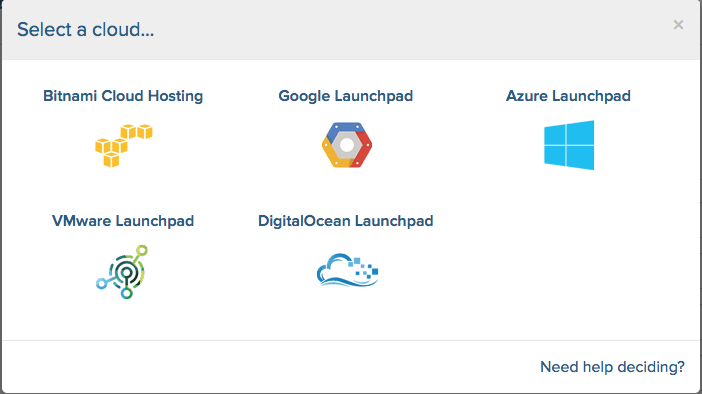
\includegraphics[width=\textwidth]{clouds}
\subsubsection{Bitnami Cloud Hosting}

\subsubsection{Digitalocean Launchpad}
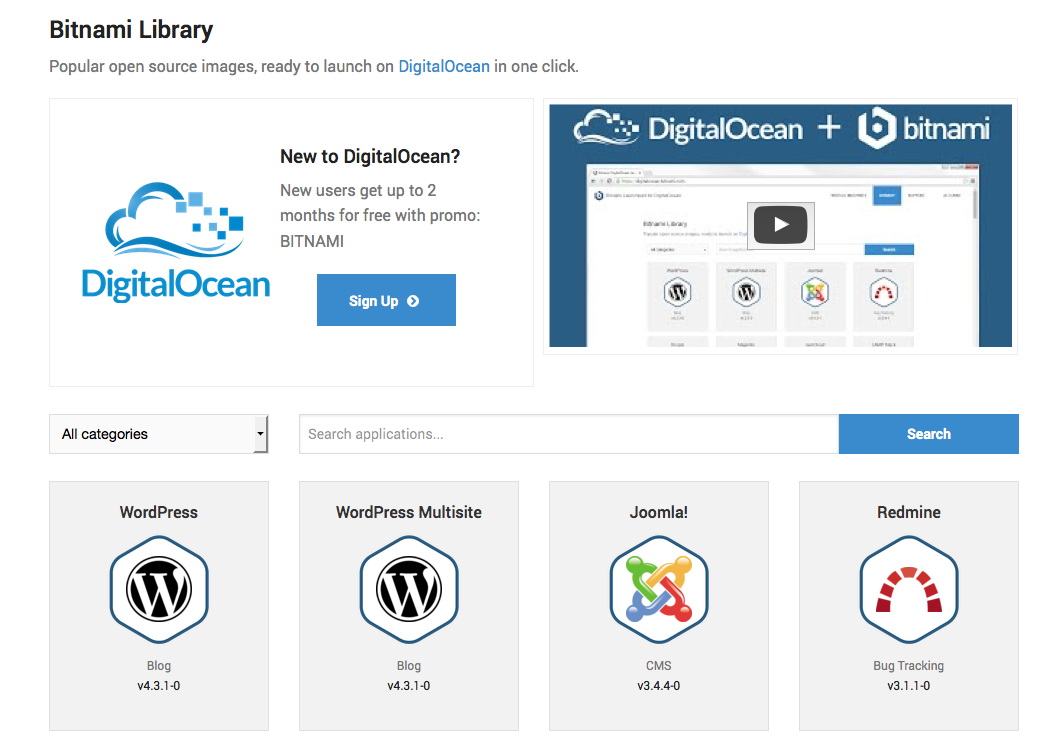
\includegraphics[width=\textwidth]{digitalocean_launchpad}
\textbf{Instanzen:}
Sobald eine Applikation ausgewählt wurde kann eine Instanz mit dem App gestartet 
werden, dabei kann noch die Instanzgrösse und Location gewählt werden.



\subsubsection{Google Launchpad}

\subsubsection{Azure Launchpad}

\subsubsection{VMware Launchpad}


\subsection{Applikationen}
Die Applikationen können sich von Anbieter zu Anbieter unterscheiden, jedoch 
gibt es für sehr viel verwendete Applikationen (Bspw.: Wordpress) bei jedem ein 
Image.
Es besteht bereits eine sehr grosse Auswahl für sehr viel verschiedene Apps und 
es werden immer mehr, wodurch es immer einfacher wird schnell eine Applikation 
aufzusetzen.
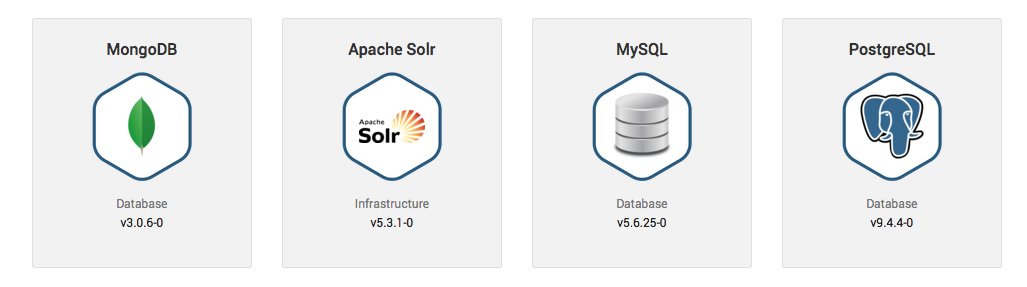
\includegraphics[width=\textwidth]{apps}

\subsubsection{Kategorien}
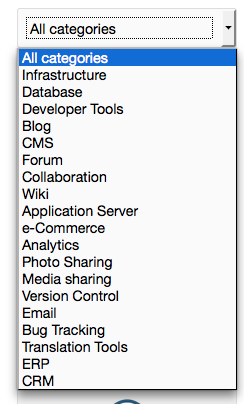
\includegraphics[width=0.5\textwidth]{categories}

\end{document}